\documentclass[12pt, letterpaper, parskip = full]{article}
\usepackage{datetime2}

\usepackage[utf8]{inputenc}
\usepackage{amsmath}
\usepackage{mathpazo}
\usepackage{eulervm}

\usepackage[margin=1in]{geometry}
\linespread{1.20}
\usepackage{enumerate}
\usepackage{enumitem}
\usepackage{listings}
\usepackage[T1]{fontenc}
\usepackage{amsfonts}
\usepackage{amssymb}
\usepackage{amsthm}
\usepackage{multirow,array}
\usepackage{graphicx}
\usepackage{physics}
\usepackage{bm}
\usepackage{tikz}
\usepackage{breqn}
\usepackage[longnamesfirst]{natbib}
\usepackage{comment}
\usepackage{setspace}
\usepackage{hyperref}

\graphicspath{{Images/}}

\newtheorem{theorem}{Theorem}
\newtheorem{corollary}{Corollary}
\newtheorem{lemma}{Lemma}
\newtheorem{definition}{Definition}
\newtheorem{axiom}{Axiom}
\newcommand{\e}{\mathrm{e}}
\newcommand{\Var}{\mathrm{Var}}
\newcommand{\Ex}[1]{\mathbb{E}\left[#1\right]}
\renewcommand{\Pr}[1]{\mathbb{P}(#1)}
\newcommand{\plim}{\mathrm{plim}}
\newcommand{\pc}[1]{\frac{\dot{#1}(t)}{#1(t)}}
\renewcommand\qedsymbol{$\blacksquare$}

\title{Homework 7}
\author{Alejandro Flores-Brown}
\date{04/12/2019}


\begin{document}

  \maketitle

  \section{Problem 1 Part A}

  Firms find the high-productivity state more valuable because they produce more and then earn more. The firm also employs more people, as their marginal product is higher; this is suggested by elementary analysis of the production function. High-value firms always want to stay in the market, while lower-valued firms are unlikely to stay in the market unless they have many workers, in which case they may not want to pay the large fixed cost associated with exiting and firing all employees.

  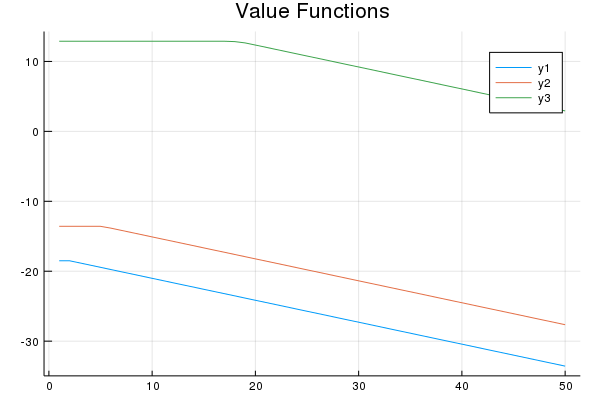
\includegraphics[scale=0.25]{val.png}
  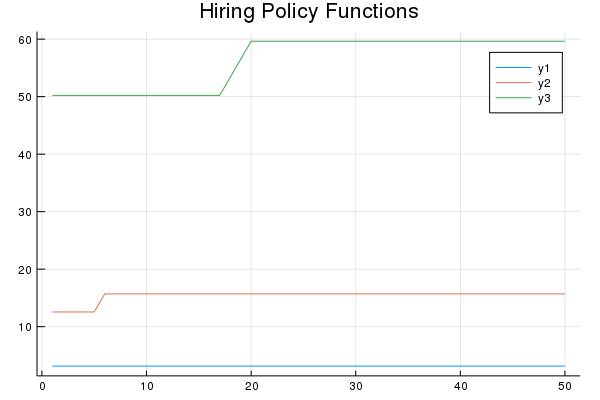
\includegraphics[scale=0.25]{npol.png}
  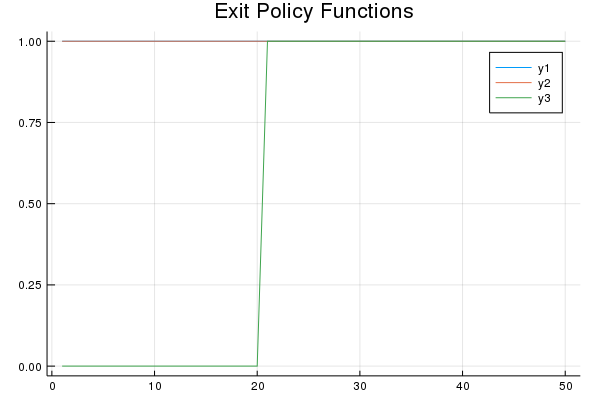
\includegraphics[scale=0.25]{xpol.png}

  \section{Problem 1 Part B}

  The equilibrium prices are $p(40) = 1.216$, $p(30) = 1.162$, and $p(50) = 1.259$. The value of entering the market increases as the price increases. This is because when the price increases, the marginal profit of firms increases, and thus entry becomes more valuable. The price is also increasing as the entry cost increases. This implies that when the entry cost increases, the total supply of goods in the market is less because there are less firms in equilibrium, increasing the price.

  \section{Problem 1 Part C}

  Code to calculate the distribution is included, but there appears to be an error. In any case, I cannot figure out how to produce the plot.

  \section{Problem 1 Parts D and E}

  Decreasing the number of entrants decreases the total output of the economy and employment, as there are less firms. The exit rate also decreases, as there are less entrants, and so the equilibrium price and thus equilibrium profits increases.

  \begin{table}[]
  \begin{tabular}{|l|l|l|}
  \hline
             & m=0.1 & m=0.00165                   \\ \hline
  Entry      & 0.1   & $1*10^{-7}$    \\ \hline
  Exit       & 0.354 & 0.340                       \\ \hline
  Adj. Costs & 0     & 0                           \\ \hline
  Output     & 5.58  & $5.58*10^{-6}$ \\ \hline
  Employment & 6793  & 5695                        \\ \hline
  \end{tabular}
  \end{table}

  \section{Problem 2 Part A}

  Decreasing $\delta$ appears to increase employment, output, and exit. Because firms can exit at less cost, they are more willing to exit. Consequently, the exit rate rises. Employment increases because firms are more willing to hire workers because firing them is less costly. Accordingly, output rises because more people are working.

  \begin{table}[]
  \begin{tabular}{|l|l|l|}
  \hline
             & m=0.02 & m=0.0017 \\ \hline
  Entry      & 0.02   & 0.0017   \\ \hline
  Exit       & 0.3389 & 0.123    \\ \hline
  Adj. Costs & 0      & 0        \\ \hline
  Output     & 1.158  & 0.091    \\ \hline
  Employment & 10833  & 6039     \\ \hline
  $\delta$      & 0      & 0.02     \\ \hline
  \end{tabular}
  \end{table}

  \section{Problem 2 Part B}

  I suspect that there is a fatal error in the code, so I compare the economy holding exit constant to attempt to compensate for this. Decreasing the persistence of the shock appears to decrease employment, increase output, and increase exit. Because productivity is less persistent, firms are more likely to hit a state in which they exit (because incumbents are less likely to keep high productivity). Because high-productivity firms are less likely to want to keep the same level of employment, they hire less workers and thus decrease employment in equilibrium so as to decrease the risk from firing costs. However, output increases because low-productivity firms are more willing to enter and hire workers because the likelihood of becoming more productive increases.

  \begin{table}[]
\begin{tabular}{|l|l|l|}
\hline
           & m=0.10 & m=0.10 \\ \hline
Entry      & 0.10   & 0.10   \\ \hline
Exit       & 0.192  & 0.235  \\ \hline
Adj. Costs & 0      & 0      \\ \hline
Output     & 32.5   & 43.9   \\ \hline
Employment & 9396   & 9156   \\ \hline
$\rho$        & 0.75   & 0.5    \\ \hline
\end{tabular}
\end{table}

\newpage

\appendix

Julia Code

 \begin{lstlisting}[breaklines]
 using Distributions, LinearAlgebra, Plots

 const alpha = 2/3
 const r = 0.2
 const delta = 0.1
 const delta1 = 0.0
 const delta2 = 0.2
 const cf = 20
 const ce = 40
 const ce1 = 30
 const ce2 = 50
 const theta = 100
 #const rho = 0.9
 #const rho = 0.75
 const rho = 0.5
 const p_in = 0.9
 const lz = 1.39
 const sigma = 0.2
 const lambda = 1
 const z_length = 5
 const tol = 0.00001
 const h = 0.0001

 D(p) = theta/p


function Tauchen(lambda::Number, m::Number, rho::Number, sigma::Number, mu::Number)
    #discretize AR(1) Process
    local z1 = mu - lambda * sigma * (1-rho)^(-0.5)
    local step = -2*z1*(m-1)^(-1)
    local zm = z1 + (m-1)*step
    local AR1 = collect(range(z1, length=m, stop=zm))

     #Compute transition matrix
     local TransMat = zeros(m,m)
     local quant

     for j=1:m
         for k=1:m

             quant=0
             if k==1
                 quant = cdf(Normal(), ((AR1[k] + 0.5*step - rho*AR1[j])/sigma) )
             elseif k==m
                 quant = 1 - cdf(Normal(), ((AR1[k] - 0.5*step - rho*AR1[j])/sigma) )
             else
                 quant = cdf(Normal(), ((AR1[k] + 0.5*step - rho*AR1[j])/sigma) ) - cdf(Normal(), ((AR1[k] - 0.5*step - rho*AR1[j])/sigma) )
             end
             TransMat[j,k] = quant
         end
     end

     return AR1, TransMat
 end

 zp = Tauchen(lambda,z_length,rho,sigma,0)
 z = zeros(z_length)
 Gamma = zp[2]

 for i=1:z_length
   z[i] = exp(zp[1][i]+1.39)
 end
 G = (1/z_length)*ones(z_length)

 #m_in = (1/z_length)*ones(z_length)
 #m_plus = transpose(m_in)*Gamma
 #m_star = transpose(m_in)*(Gamma^1000)


 nmin = 0.0
 nmax = alpha*0.9*z[z_length]^(1/(1-alpha))
 n_length = 50
 n = collect(range(nmin, length=n_length, stop=nmax))

 V_0 = zeros(n_length, z_length)

 V(i,j,k,Vold,p,delta) = p*z[i]*n[k]^alpha - n[k] - delta*max(n[j]-n[k],0) - cf + (1/(1+r))*dot(Gamma[i,:],max.(Vold[:,k],-delta*n[k]))
 Ve(ce,V) = -ce + (1/(1+r))*dot(G,max.(V[:,1],0))

 function solveBell(p::Number,delta::Number)
   local Vold = zeros(z_length, n_length)
   local Vnew = zeros(z_length, n_length)
   local Vind = zeros(z_length, n_length)
   local Vtemp = zeros(n_length)
   local diff = 0

   while true
     for i=1:z_length
       for j=1:n_length
         for k=1:n_length
           Vtemp[k] = V(i,j,k,Vold,p,delta)
         end
         Vnew[i,j] = maximum(Vtemp)
         Vind[i,j] = argmax(Vtemp)
         Vtemp = zeros(n_length)
       end
     end

     diff = maximum(Vnew-Vold)
     if diff < tol
       Vind = convert(Array{Int,2},Vind)
       break
     end

     Vind = zeros(z_length, n_length)
     Vold = zeros(z_length, n_length)
     Vold = Vnew
     Vnew = zeros(z_length, n_length)
   end

   n_pol = zeros(z_length, n_length)
   x_pol = ones(z_length, n_length)
   for i=1:z_length
     for j=1:n_length
       V_aux = zeros(z_length, n_length)
       V_aux[i,j] = max(Vnew[i,Vind[i,j]],-delta*n[Vind[i,j]])
       if abs(V_aux[i,j] - Vnew[i,j]) < tol
         x_pol[i,j] = 0
       end
       n_pol[i,j] = n[Vind[i,j]]
     end
   end

   return Vnew, Vind, n_pol, x_pol
 end

 #Part A

 sol1 = solveBell(p_in,delta)
 Val1 = sol1[1]
 dom1 = sol1[2]
 n1 = sol1[3]
 x1 = sol1[4]


 #plot_V1 = plot([Val1[1,:] Val1[3,:] Val1[5,:]], title="Value Functions")
 #savefig("val")
 #plot_n1 = plot([n1[1,:], n1[3,:], n1[5,:]], title="Hiring Policy Functions")
 #savefig("npol")
 #plot_x1 = plot([x1[1,:], x1[3,:], x1[5,:]], title="Exit Policy Functions")
 #savefig("xpol")

 #Part B

 #ve1 = Ve(40, Val1)
 #ve2 = Ve(30, Val1)
 #ve3 = Ve(50, Val1)

 function Newton_ve(p,delta,ce)
   local p_it = 0
   local ve_f = 0
   while true
     val = solveBell(p,delta)[1]
     valh = solveBell(p+h,delta)[1]
     p_it = p - h*Ve(ce,val)/(Ve(ce,valh) - Ve(ce,val))
     if abs(p_it - p) < tol
       break
     end
     p = 0
     p = p_it
     p_it = 0
   end
   return p_it
 end

 #p1 = Newton_ve(p_in,delta,ce)
 #p2 = Newton_ve(p_in,delta,ce1)
 #p3 = Newton_ve(p_in,delta,ce2)

 #Part c

 function lambda(m0::Number, delta::Number, ce::Number)
   p_star = Newton_ve(1.2,delta,ce)
   sol = solveBell(p_star, delta)
   val = sol[1]
   domv = sol[2]
   npol = sol[3]
   xpol = sol[4]

   In = zeros(z_length, n_length)
   In_n = zeros(z_length,n_length,n_length)

   for i=1:n_length
     if n[i]==0
       In[i] = 1
     end
   end

   for i=1:z_length
     for j=1:n_length
       for k=1:n_length
         if npol[i,j] == n[k]
           In_n[i,j,k] = 1
         end
       end
     end
   end

   lambda0 = ones(z_length, n_length, 1, 1)
   lambda1 = zeros(z_length, n_length, z_length, n_length)
   lambdaret = zeros(z_length, n_length, 1, 1)
   while true
     for i=1:z_length
       for j=1:n_length
         for k=1:z_length
           for l=1:n_length
             lambda1[i,j,k,l] = lambda0[k,l,1,1]*(1-xpol[k,l]) * Gamma[k,i]*In_n[k,l,j] + m0*G[i]*In[j]
           end
         end
       end
     end

     lambdat1 = sum(lambda0, dims=4)
     lambdaret = sum(lambdat1, dims=3)
     if abs(maximum(lambdaret - lambda0))<tol
       break
     else
       lambda0 = zeros(z_length, n_length, 1, 1)
       lambda0 = lambdaret
       lambda1 = zeros(z_length, n_length, z_length, n_length)
       lambdaret = zeros(z_length, n_length, 1, 1)
     end
   end
   return lambdaret, lambda1, npol, xpol
 end

 solc = lambda(0.10, delta, ce)
 cca = solc[1]
 ccb = solc[2]
 ccc = solc[3]
 ccd = solc[4]

 lambdaplot = zeros(z_length, n_length)
 for i=1:z_length
   for j=1:n_length
     lambdaplot[i,j] = ccb[i,j,1,1]
   end
 end

 #Part d
 function compstats(trans::Array{Float64,4}, otrans::Array{Float64,4}, npol::Array{Float64,2}, xpol::Array{Float64,2})
 Q1 = zeros(z_length, n_length)
 Q2 = zeros(z_length, n_length)
 for i=1:z_length
   for j=1:n_length
     Q1[i,j] =  otrans[i,j,1,1] * z[i] *npol[i,j]^alpha * (1 - xpol[i,j])
     Q2[i,j] = otrans[i,j,1,1] * z[i] * npol[i,j]^(alpha-1) * (1 - xpol[i,j])
   end
 end

 sQ1 = sum(Q1)
 sQ2 = sum(Q2)
 total = sum(otrans)
 exit = sum(otrans.*xpol)/total
 L = sum(otrans.*npol.*(ones(z_length, n_length)-xpol))

 adjc = zeros(z_length,n_length)
 for i=1:z_length
   for j=1:n_length
     adjc = otrans[i,j,1,1] * delta * max(n[j]-npol[i,j],0)*(1-xpol[i,j])
   end
 end
 tadjc = sum(adjc)

 return sQ1, sQ2, total, exit, L, tadjc
 end


 #use this again for Problem 2 Part b with appropriate rho

 stats14 = compstats(cca, ccb, ccc, ccd)
 #Question 2

 #part a

 sol2_1 = lambda(0.02, delta1, ce)
 sol2_1s = compstats(sol2_1[1], sol2_1[2], sol2_1[3], sol2_1[4])

 sol2_2 = lambda(0.0017, delta2, ce)
 sol2_2s = compstats(sol2_2[1], sol2_2[2], sol2_2[3], sol2_2[4])

 \end{lstlisting}

\end{document}
